\documentclass[hyperref={pdfpagelayout=SinglePage}]{beamer}

%Template
\usetheme{Warsaw}
\usecolortheme{default}
\usefonttheme[onlymath]{serif}

%Packages
\usepackage[utf8]{inputenc}
\usepackage[spanish,activeacute]{babel}
\usepackage{lipsum}
\usepackage{graphicx}
\usepackage{fancyhdr}
\usepackage{float}
\usepackage{adjustbox}
\usepackage{subfigure}
\usepackage{amsmath}
\usepackage{ragged2e}
\usepackage{color}
\usepackage{listings}
\usepackage{animate}
\usepackage{hyperref}

%Code
\lstset{ %
basicstyle=\small,       % the size of the fonts that are used for the code
numbers=none,                   % where to put the line-numbers
numberstyle=\footnotesize,      % the size of the fonts that are used for the line-numbers
stepnumber=1,                   % the step between two line-numbers. If it is 1 each line will be numbered
numbersep=5pt,                  % how far the line-numbers are from the code
backgroundcolor=\color{white},  % choose the background color. You must add \usepackage{color}
showspaces=false,               % show spaces adding particular underscores
showstringspaces=false,         % underline spaces within strings
showtabs=false,                 % show tabs within strings adding particular underscores
frame=single,           % adds a frame around the code
tabsize=4,          % sets default tabsize to N spaces
captionpos=b,           % sets the caption-position to bottom
breaklines=true,        % sets automatic line breaking
breakatwhitespace=false,    % sets if automatic breaks should only happen at whitespace
escapeinside={\%*}{*)}          % if you want to add a comment within your code
}

%Captions
\renewcommand{\lstlistingname}{Código}
\renewcommand\spanishtablename{Tabla}
\renewcommand{\figurename}{Gráfico}

%More
\makeatletter
\@addtoreset{subfigure}{framenumber}
\makeatother

\expandafter\def\expandafter\insertshorttitle\expandafter{%
  \insertshorttitle\hfill%
  \insertframenumber\,/\,\inserttotalframenumber}

\newcommand\Wider[2][5em]{%
\makebox[\linewidth][c]{%
  \begin{minipage}{\dimexpr\textwidth+#1\relax}
  \raggedright#2
  \end{minipage}%
  }%
}

%List of parts
\makeatletter
\AtBeginPart{%
    \addtocontents{parttoc}{\protect\beamer@partintoc{\the\c@part}{\beamer@partnameshort}{\the\c@page}}%
    \frame{\partpage}%
}
\newcommand{\parttableofcontents}{\@starttoc{parttoc}}
\newcommand{\beamer@partintoc}[3]{#2\par}
\makeatother

%Document Data
\title{Medios Granulares}
\subtitle{Trabajo Práctico Nro. 5}
\author{Badi Leonel, Buchhalter Nicolás Demián y Meola Franco Román}
\subject{Simulación de Sistemas}
\date{\today}

\begin{document}

%Part List
%\frame{\frametitle{Que vamos a ver}\parttableofcontents}

%First Part
%\part{Oscilador Puntual Amortiguado}

\begin{frame}[plain]
    \frametitle{} 
    \titlepage
    \centering
	Grupo 3
\end{frame}

\section{Fundamentos}

\subsection{Introducción}

\begin{frame}
\frametitle{Fundamentos}
\framesubtitle{Introducción}
\begin{itemize}
	\item Vamos a simular un medio granular gravitatorio que fluye desde un silo
	\item El silo bidimensional está definido por:
	\begin{itemize}
		\item \textbf{Ancho} $W$
		\item \textbf{Altura} $L$
		\item Ancho de \textbf{apertura} de la cara inferior $D$
		\item \textbf{Caída} debajo de la cara inferior de $1m$
	\end{itemize}
	\item Usaremos dinámica molecular regida por el paso temporal con un medio granular
\end{itemize}
\end{frame}

\subsection{Variables relevantes}

\section{Implementación}

\subsection{Generación de las partículas}

\begin{frame}
\frametitle{Implementación}
\framesubtitle{Generación de las partículas}
\begin{itemize}
	\item Posiciones $(x,y)$ aleatorias
	\begin{itemize}
		\item Verificando que no se superpongan
		\item Intentando hasta 10000 veces por partícula para obtener una ubicación válida 
	\end{itemize}
	\item $D = 1$
	\item $r = \frac{D}{20}$
	\item $v_{0} = 0$
\end{itemize}
\end{frame}

\subsection{Simulación}

\begin{frame}
\frametitle{Simulación}
\framesubtitle{Variables relevantes del sistema}
\begin{itemize}
	\item $k_{N} = 10^5 \frac{N}{m}$
	\item $k_{T} = 2 k_{N}$
	\item $m = 0.01 kg$
\end{itemize}
\end{frame}

\begin{frame}
\frametitle{Simulación}
\framesubtitle{Variables relevantes de la simulación}
\begin{itemize}
	\item $t$: tiempo en segundos a visualizar
	\item $dt$: tiempo en segundos del paso de simulación
	\item $k$: relación entre cantidad de pasos simulados y escritos.
\end{itemize}
\end{frame}

\begin{frame}[fragile]
\frametitle{Simulación}
\framesubtitle{Algoritmo de simulación}
\begin{lstlisting}[language=Java, caption = Algoritmo de simulación]
public void simulate(double t, double dt, int k){
	granularSystem.writeFrame(0);
    int framesWrited = 1;
    double totalTimeSimulated = 0;
    granularSystem.move(dt);
    totalTimeSimulated += dt;
    while(totalTimeSimulated < t){
		for(int i = 0; i < k; i++){
			granularSystem.move(dt);
        	totalTimeSimulated += dt;
    	}
    	granularSystem.writeFrame(framesWrited++);
    }
}
\end{lstlisting}
\end{frame}

\begin{frame}
\frametitle{Simulación}
\framesubtitle{Problemas encontrados}
\begin{itemize}
	\item Velocidades muy altas de las partículas debido a que no se estaba invirtiendo el ángulo de la normal cuando las mismas colisionaban.
	\item Valores de \textit{overlap} muy altos en las inmediaciones a los bordes del silo.
	\item Con un valor de $\Delta t$ del orden del sugerido en la teórica ($0.1 \sqrt{\frac{m}{K_{n}}}$), obtuvimos malos resultados:
	\begin{itemize}
		\item Utilizando \textit{Beeman} como método de integración
		\item No se detectaban correctamente las colisiones a tiempo
		\item Ocasionaba la pérdida de una gran cantidad de partículas
	\end{itemize}
\end{itemize}
\end{frame}

\begin{frame}
\frametitle{Simulación}
\framesubtitle{Detalles de implementación}
\begin{itemize}
	\item Se utiliza \textit{Euler} como método integrador para todos los pasos de la simulación
	\item Se utiliza \textit{Cell Index Method} para el manejo de colisiones de las partículas 
\end{itemize}
\end{frame}

\subsection{Visualización}

\begin{frame}
\frametitle{Implementación}
\framesubtitle{Visualización}
\begin{itemize}
	\item La simulación y la visualización son independientes
	\item El algoritmo de simulación escribe un archivo \texttt{.tsv} con los siguientes datos:
	\begin{itemize}
		\item $(x,y)$
		\item $r$
		\item Color RGB para indicar las velocidades, donde R es la componente en el eje Y y G es la componente en eje X
	\end{itemize}
	\item Por último, se carga en \texttt{Ovito} el archivo de salida\texttt{.tsv} para realizar la visualización
\end{itemize}
\end{frame}

\section{Resultados}

\subsection{Gráficos y Tablas}

\begin{frame}
\frametitle{Resultados}
\framesubtitle{Variables relevantes}
\begin{itemize}
	\item \textbf{Caudal ($C$)}: número de partículas que pasan por la apertura en un instante de tiempo
	\item \textbf{Caudal medio ($C_{M}$)}: promedio del caudal para una franja temporal
	\item \textbf{Energía cinética ($E_{C}$) del sistema}: suma total de las energías de las partículas
	\item \textbf{Tiempo de relajación ($t_{r}$) del sistema}: tiempo total que le lleva al sistema de silo cerrado ($D = 0$) estabilizar su $E_{C}$
\end{itemize}
\end{frame}

\begin{frame}
\frametitle{Resultados}
\framesubtitle{$C_{M}$ para distintos valores de $L$}
\begin{center}
\begin{table}[h]
\centering
\adjustbox{max height=\dimexpr\textheight-3.0cm\relax,
           max width=\textwidth}{
\begin{tabular}{ccc}
\hline
\textbf{$L$} & \textbf{$C_{M}$}\\ \hline
3&180\\ 
7&77\\ 
10&87\\
\end{tabular}
}
\caption{$C_{M}$ para distintos valores de $L$}
\end{table}
\end{center}
\end{frame}

\begin{frame}
\Wider{
\frametitle{Resultados}
\framesubtitle{Evolución temporal de $C$ para distintos valores de $L$}
\begin{figure}[H]
	\centering
    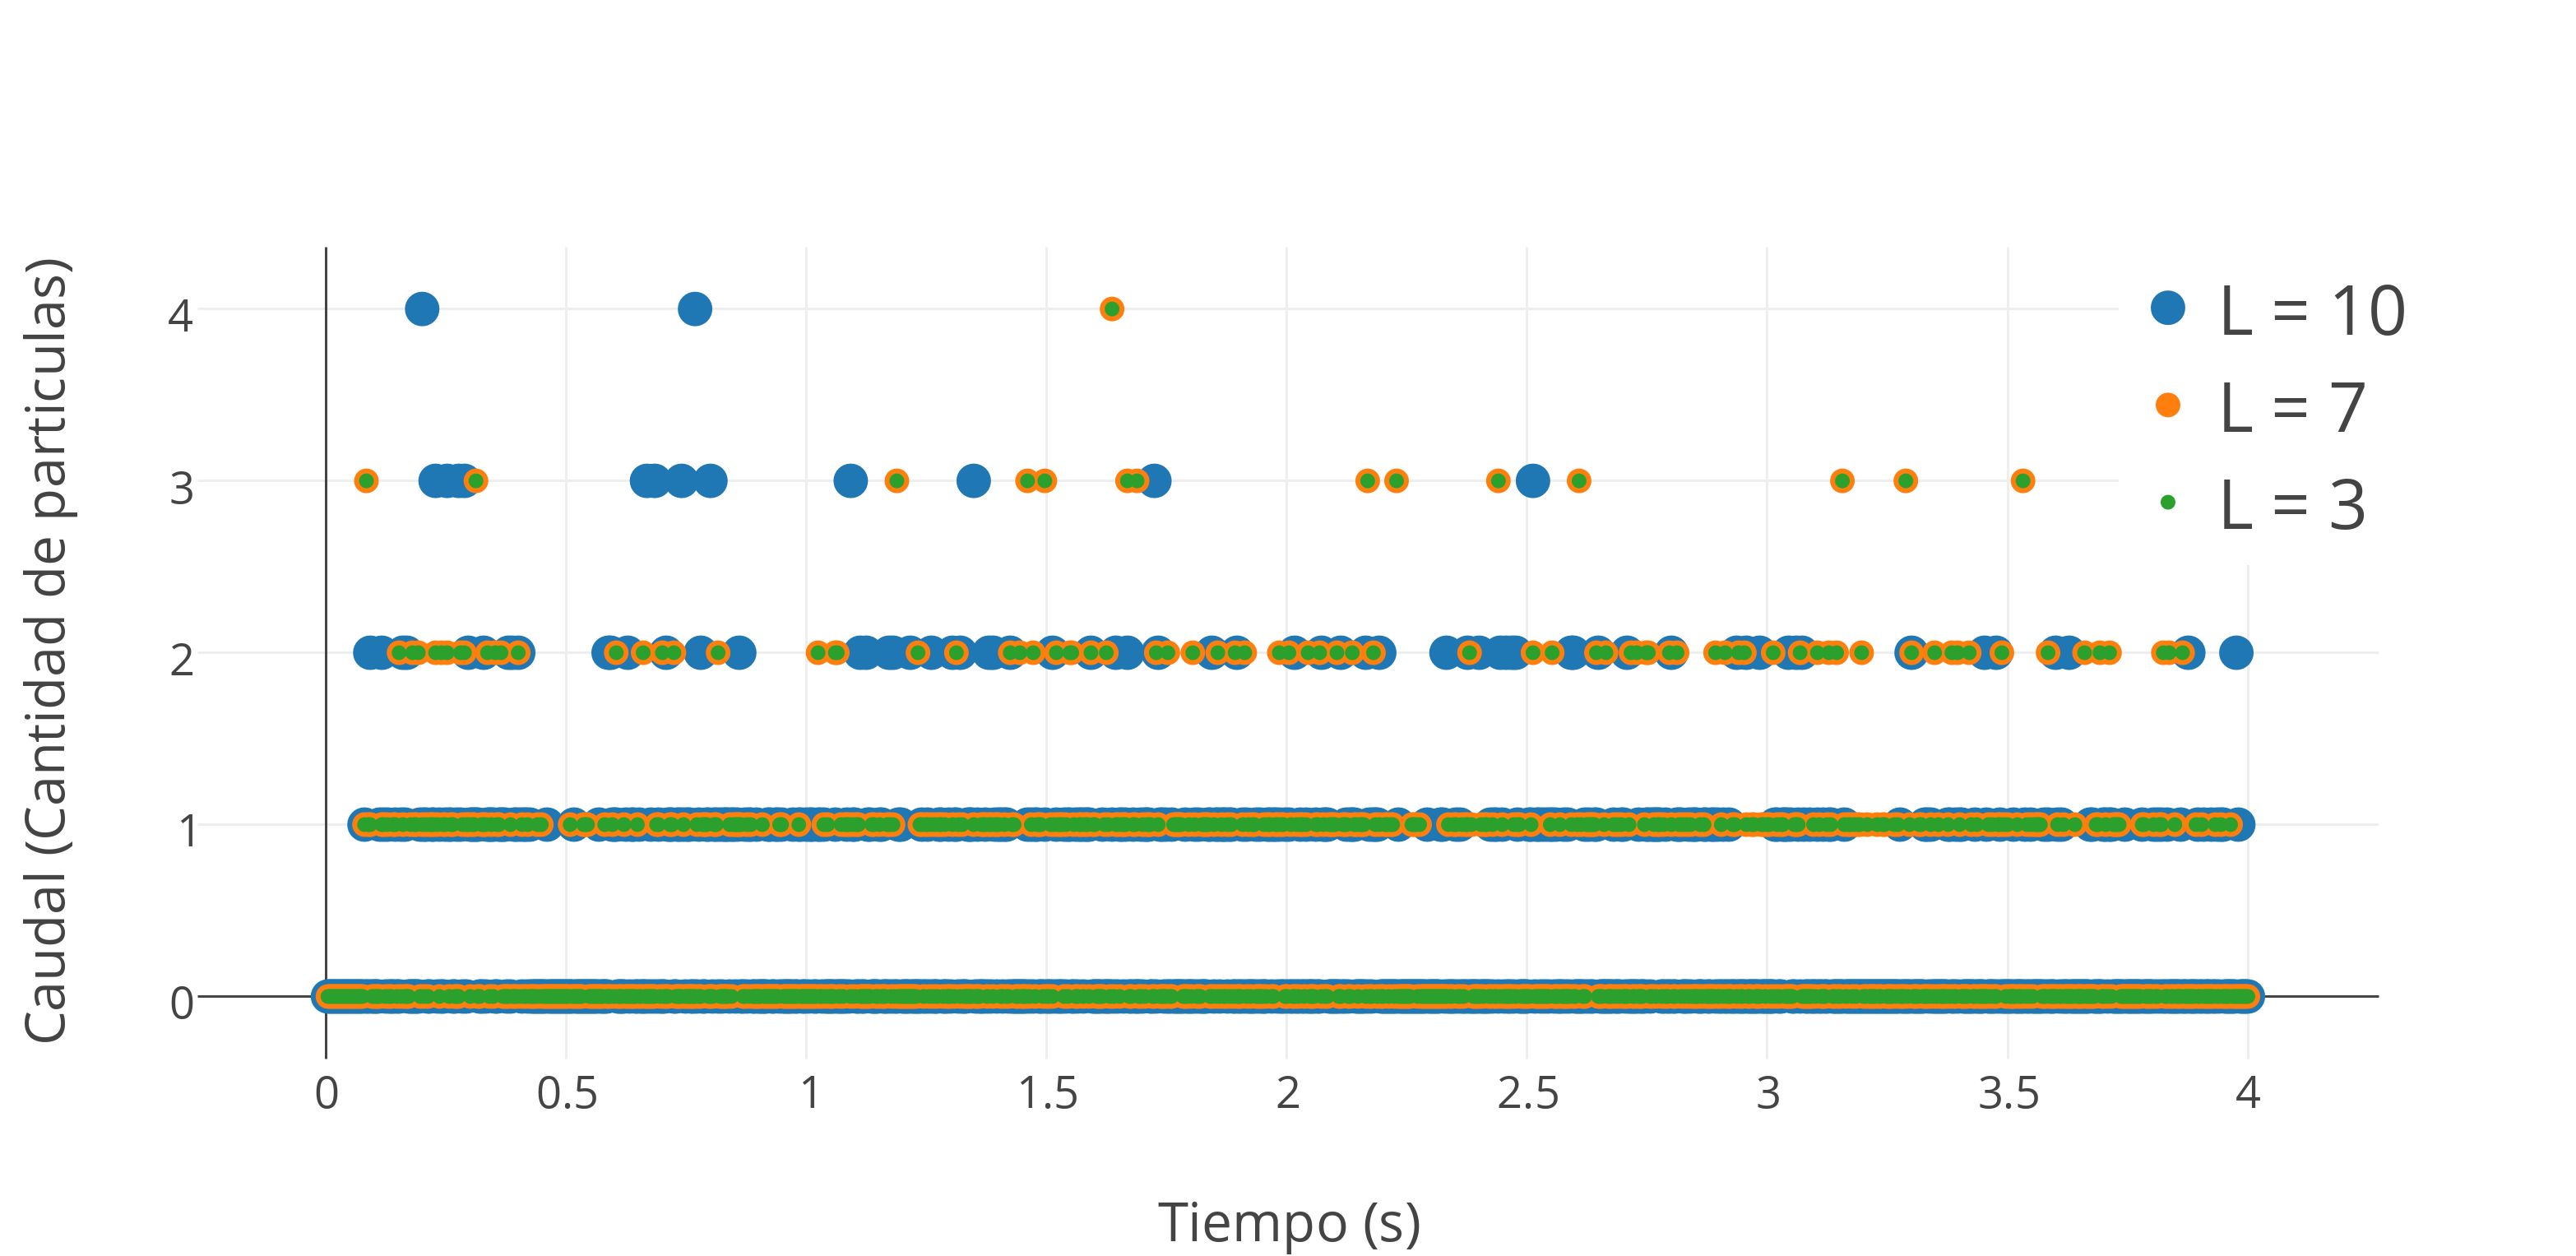
\includegraphics[width=\textwidth]{charts/caudal.png}
\end{figure}
}
\end{frame}

\begin{frame}
\Wider{
\frametitle{Resultados}
\framesubtitle{Evolución temporal de $E_{c}$ para distintos valores de $L$}
\begin{figure}[H]
	\centering
    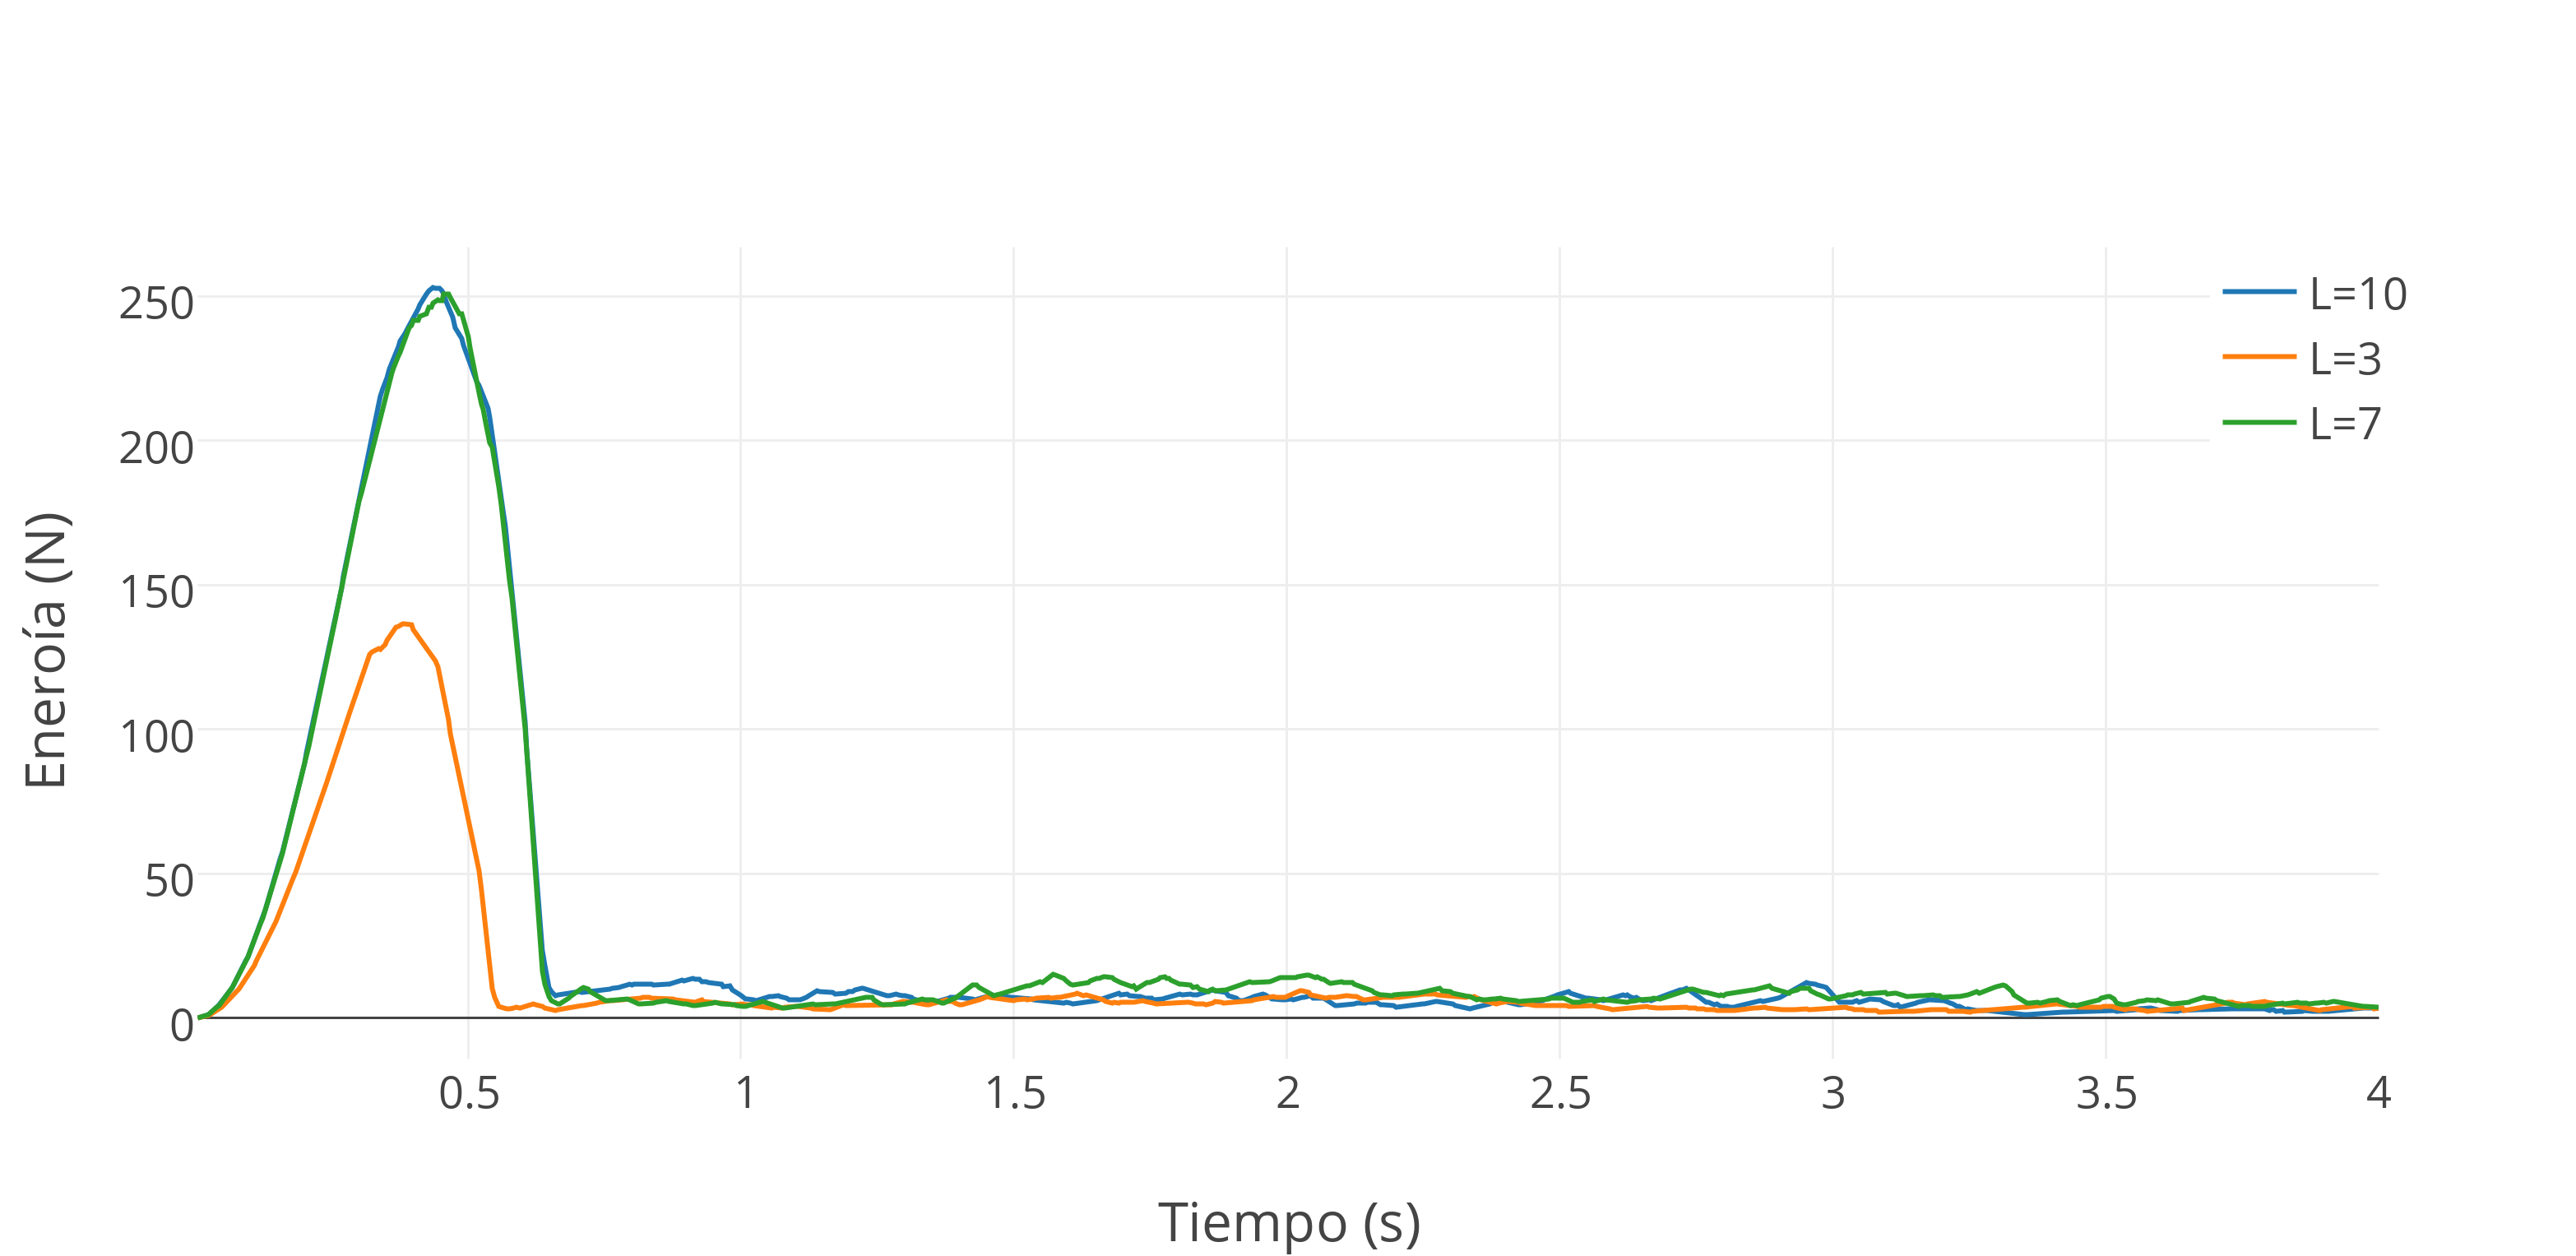
\includegraphics[width=\textwidth]{charts/energiaabierto.png}
\end{figure}
}
\end{frame}

\begin{frame}
\frametitle{Resultados}
\framesubtitle{$t_{r}$ para distintos valores de $L$}
\begin{center}
\begin{table}[h]
\centering
\adjustbox{max height=\dimexpr\textheight-3.0cm\relax,
           max width=\textwidth}{
\begin{tabular}{cc}
\hline
\textbf{$L$} & \textbf{$t_{r}$}\\ \hline
3&0.38401\\
7&0.55601\\
10&0.69601\\
\end{tabular}
}
\caption{$t_{r}$ para distintos valores de $L$}
\end{table}
\end{center}
\end{frame}

\begin{frame}
\Wider{
\frametitle{Resultados}
\framesubtitle{Evolución temporal de $E_{c}$ para el silo cerrado ($D = 0$) para distintos valores de $L$}
\begin{figure}[H]
	\centering
    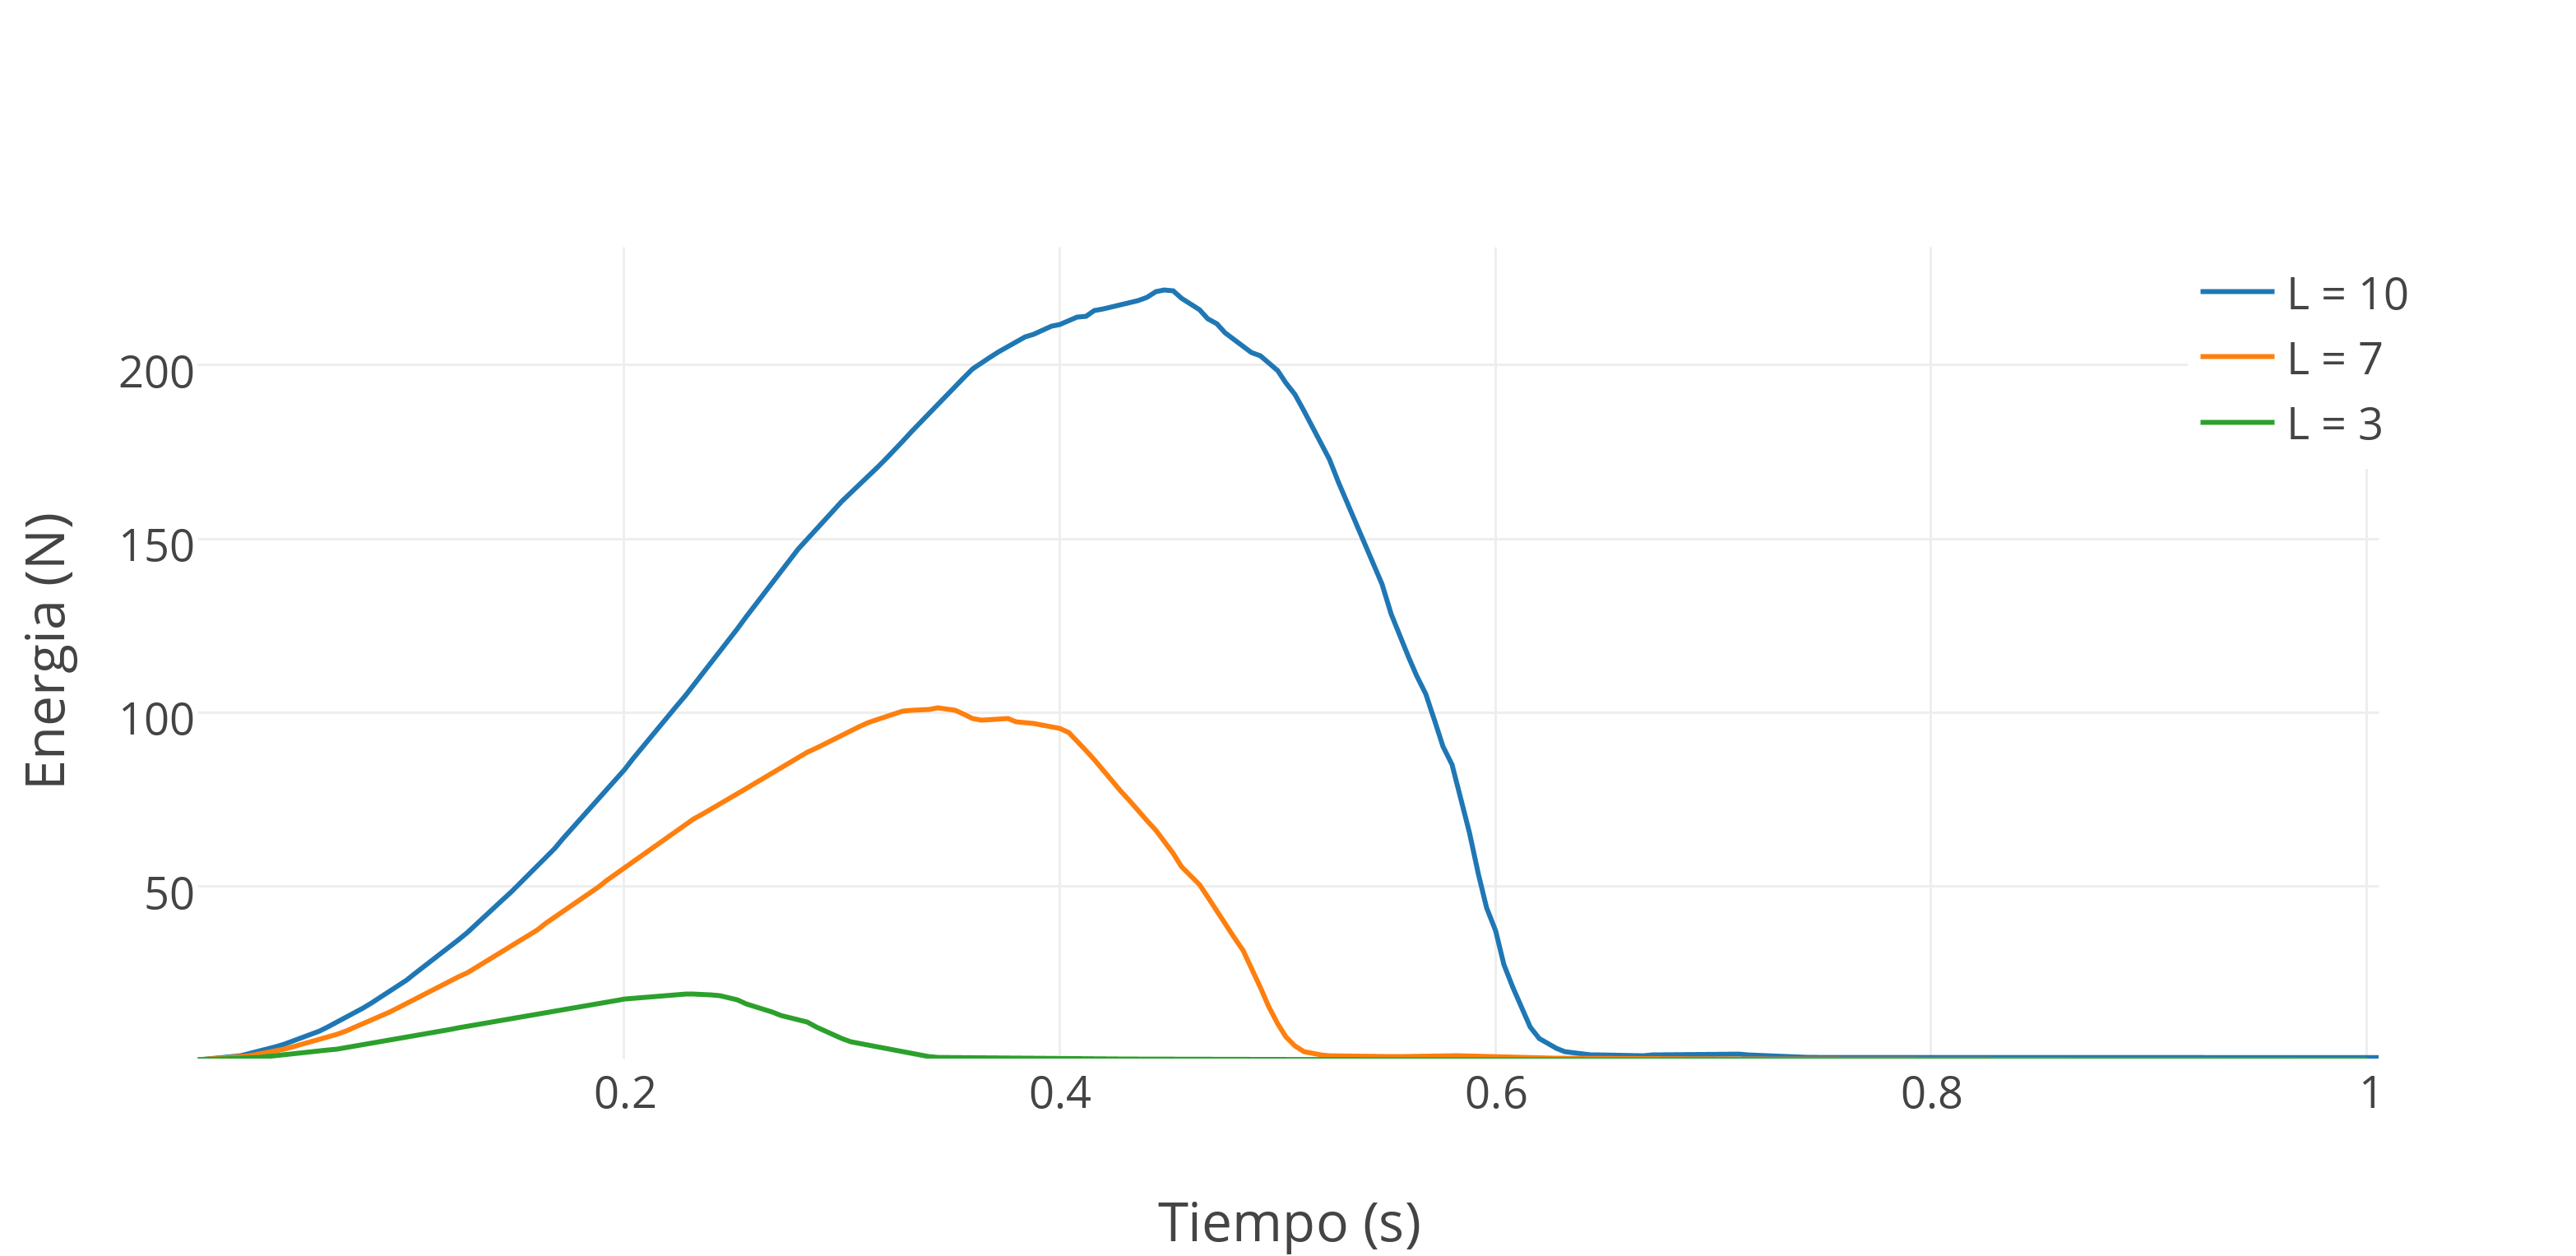
\includegraphics[width=\textwidth]{charts/energycerrado.png}
\end{figure}
}
\end{frame}

\subsection{Animaciones}

\begin{frame}[plain]
\frametitle{Resultados}
\framesubtitle{Animación de la simulación del silo para $L = 10$}
\begin{figure}[H]
	\centering
	\animategraphics[loop,controls,width=0.90\textheight]{60}{animation/completo}{00001}{00625}
\end{figure}
\end{frame}

\begin{frame}[plain]
\frametitle{Resultados}
\framesubtitle{Animación de la simulación del silo para $L = 10$}
\begin{figure}[H]
	\centering
	\animategraphics[loop,controls,width=0.90\textheight]{60}{animation/zoom}{00001}{02070}
\end{figure}
\end{frame}

\begin{frame}[plain]
\frametitle{Resultados}
\framesubtitle{Animación de la simulación del silo cerrado para $L = 10$}
\begin{figure}[H]
	\centering
	\animategraphics[loop,controls,width=0.90\textheight]{60}{animation/cerrado}{00001}{00501}
\end{figure}
\end{frame}

\subsection{Conclusiones}

\begin{frame}
\frametitle{Conclusiones}
\framesubtitle{Para el silo abierto}
\begin{itemize}
	\item Formación de arcos cerca de la apertura
	\item Una vez que el $L$ es suficientemente superior al $W$, se aprecia que el $C_{M}$ es constante (Regla de \textit{Janssen})
	\item Pérdida de solidez de la superficie
\end{itemize}	
\end{frame} 

\begin{frame}
\Wider{
\frametitle{Conclusiones}
\framesubtitle{Formación de arcos cerca de la apertura}
\begin{figure}[H]
	\centering
    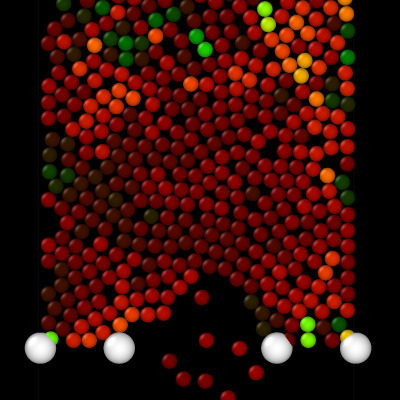
\includegraphics[width=0.75\textheight]{images/arco.png}
\end{figure}
}
\end{frame}

\begin{frame}
\Wider{
\frametitle{Conclusiones}
\framesubtitle{Pérdida de solidez de la superficie}
\begin{figure}[H]
	\centering
    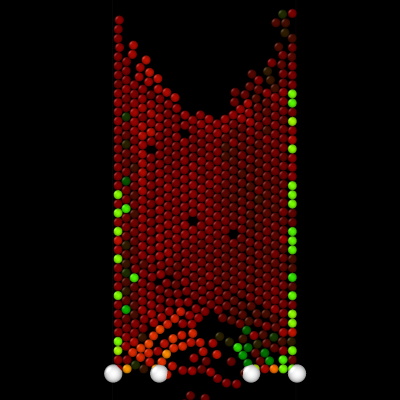
\includegraphics[width=0.75\textheight]{images/solidez.png}
\end{figure}
}
\end{frame}

\begin{frame}
\frametitle{Conclusiones}
\framesubtitle{Para el silo cerrado}
\begin{itemize}
	\item A mayor $L$, mayor $t_{r}$
	\item Se alcanza el equilibrio cuando la $E_{c}$ se mantiene constante dentro de un intervalo acotado cercano a cero
	\item Se pueden apreciar \textit{clusters} en función de la dirección de la velocidad de las partículas
\end{itemize}	
\end{frame}

\begin{frame}
\Wider{
\frametitle{Conclusiones}
\framesubtitle{\textit{Clusters} en función de la dirección de la velocidad de las partículas}
\begin{figure}[H]
	\centering
    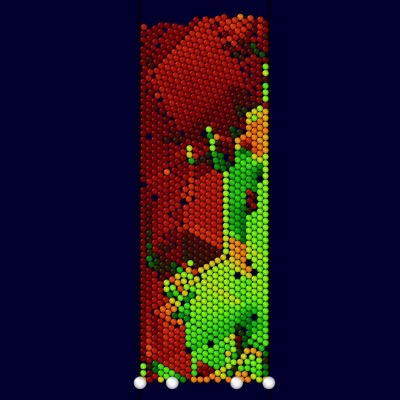
\includegraphics[width=0.75\textheight]{images/cluster.jpg}
\end{figure}
}
\end{frame}

\begin{frame}[plain]
    \centering
	\Huge Gracias
\end{frame}

\end{document}
